\documentclass[a4paper,utf8]{article}
\usepackage{exemple}
\usepackage[normalem]{ulem}
\usepackage{amsfonts}
\usepackage{graphicx}
\usepackage{MnSymbol,wasysym}
\usepackage{hyperref}
\usepackage[french]{babel}
\usepackage{graphicx}

\formation{L3MI}
\date{15/01/2017}
\matiere{Conception Orient�e Objet}
\titre{Projet : Tetris Attck }

\newcommand\code[1]{\textsf{#1}}
\newcommand\srdjan[1]{{\color{red} #1}}

\begin{document}

\entete

\begin{center}
	
\includegraphics[scale=0.9]{img1.jpg}
\end{center}

\section{Description du Projet}
Tetris Attack est un puzzle-game � 2 joueurs sorti en 1995 sur Super Nintendo. Ce jeu est une variante du bien connu Tetris � 2 joueurs. Dans cette version, l'objectif est d'assembler des blocs entre eux afin de les faire disparaitre avant que l'ensemble des blocs n'atteignent le haut de l'ecran. Toutefois, ici, 2 joueurs s'affrontent en parallele et peuvent � l'aide de diff�rentes combinaisons envoyer de nouveaux blocs de briques � leur adversaire afin de pr�cipiter sa perte. Ce jeu couple � la fois, la simplicit� de Tetris � la dynamicit� n�cessaire d'un bon Versus.

\section{L'Organisation }

\subsection{Gantt}
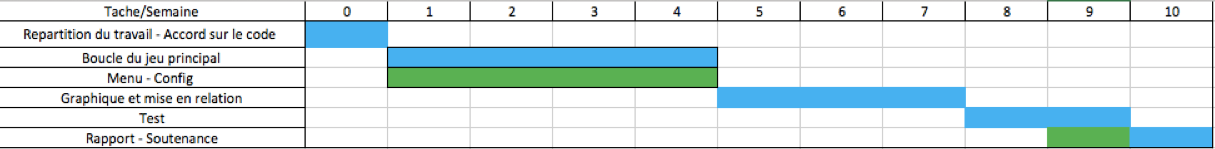
\includegraphics[scale=0.9]{gant.png}

\subsection{L'Equipe}
\begin{itemize}
\item vincent : jeu principal , graphique , ia 
\item loick : jeu principal , graphique , ia 
\item mohammed: menu , diff�rent ecrans pour config , graphique
\item kevin: menu , diff�rent ecrans pour config , graphique
\end{itemize}


\subsection{Les Moyens de Communication}
\begin{itemize}
\item les t�ches ainsi que les r�gles de codage internes au groupe seront marqu�es sur une feuille individuelle faite par chaque personne lors d'une entrevue. Ces r�gles seront instaur�s selon un point de l'�quipe avant le projet (semaine 1).
\item le projet aura des mini-deadline qui seront fait sur git avec les milestones pour un suivie pas � pas du projet ce qui va permettre de voir si l'�quipe � de l'avance ou du retard vis � vis du gant de d�part.
\item des mini-r�unions auront lieu pour savoir si telle ou telle personne est bloqu�e sur un point sachant que le projet est divis� en 2 groupes de 2 cela doit rarement arriv�. 
\item un canal de discussion sur slack a �t� cr�� sp�cialement pour notre groupe pour permettre la communication lors du travail personnel chez nous et de poser des questions Mr Piette.
\end{itemize}

\section{Le rendu du Projet }

\subsection{Les ecrans de Jeux}
\begin{center}
	
\includegraphics[scale=0.4]{img1.jpg}
\end{center}


\subsection{Le Menu}
\begin{center}
	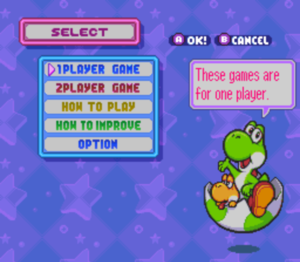
\includegraphics[scale=0.6]{img2.png}
\end{center}

\subsection{L'ecran de jeu}
\begin{center}
	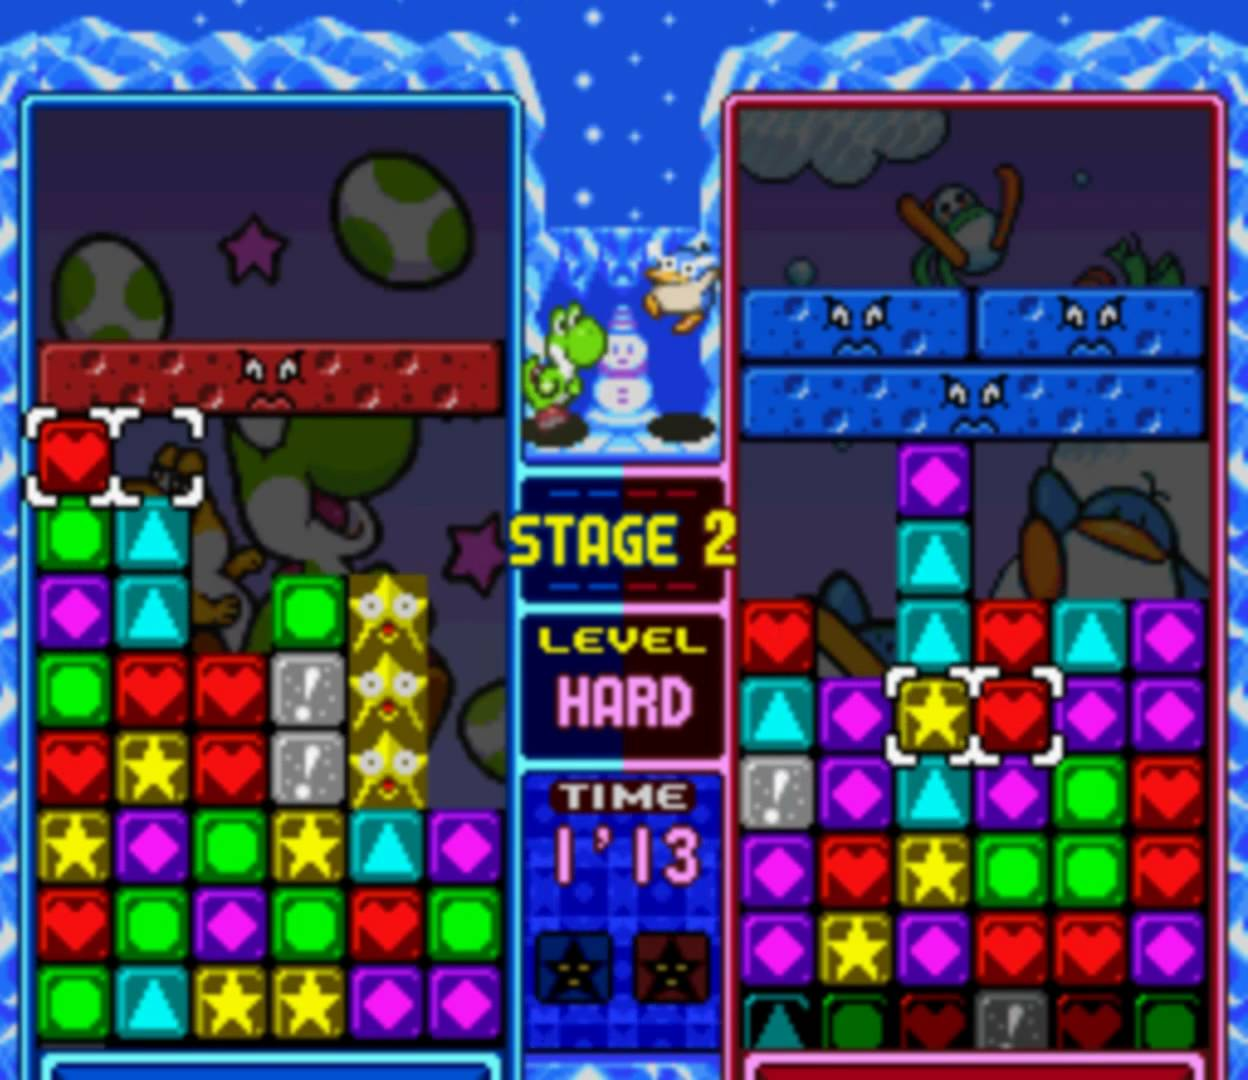
\includegraphics[scale=0.15]{img3.jpg}
\end{center}

\end{document}